\section{Results and Discussion} 
\label{sec:results}
\subsection{2D array of optical traps}
We have, $|A_{source}|^2$ as shown in 5(a) while figure 5(b) shows the targeted intensity distribution ($ |A_{target}|^2 $) having a 3x3 array of tightly focused beam of optical tweezers. Using the GS algorithm, we have iteratively find the phase $\phi_{mn}$ described in equation \ref{eq:discrete_A_slm} from the random phase shown in Figure 6(a).
\begin{figure}[H]
\centering
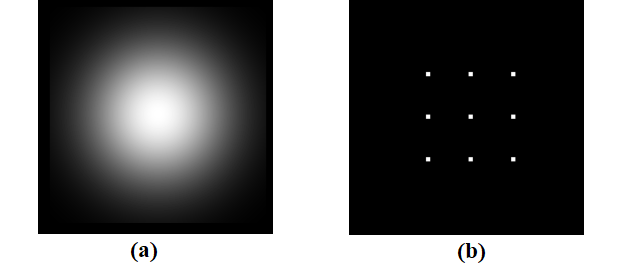
\includegraphics[width=\textwidth]{img/Target.png}
\label{fig:img_target}
\caption{(a) Source intensity distribution, (b) Target intensity distribution}
\end{figure}

\begin{figure}[H]
\label{fig:phase}
\centering
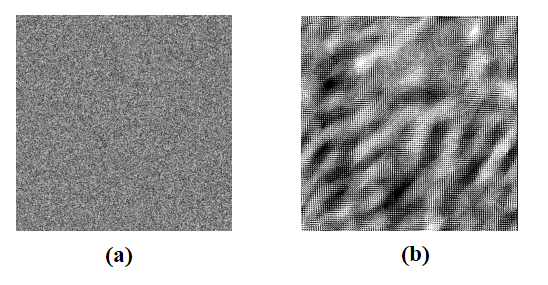
\includegraphics[width=0.91\textwidth]{img/Phase.png}
\caption{(a) Random phase, (b)Phase determined using GS Algorithm}
\end{figure}

The focal plane of the lens is imaged using a CMOS sensor which initially contains the higher diffraction order, as shown in Figure 7, so we have used the iris to select the single order and obtained the targeted intensity image. Since the SLM has a fill factor of approximately 90\%, a small portion of the reflected beam is unmodulated and appears as a bright spot in the beam's centre. We have tried to remove the unmodulated beam using the concept of the virtual lens as described in paper \cite{10.3389/fphy.2021.587112}. Nevertheless, it is not eradicated. So, we have tried to keep the array slightly far from the centre of the SLM in order to block the unmodulated beam with the iris. Figure 8(a) shows the array of tweezers imaged through the CMOS Camera, and figure 8(b) shows the intensity pattern on the screen. 

\begin{figure}[H]
\label{diff_order}
\centering
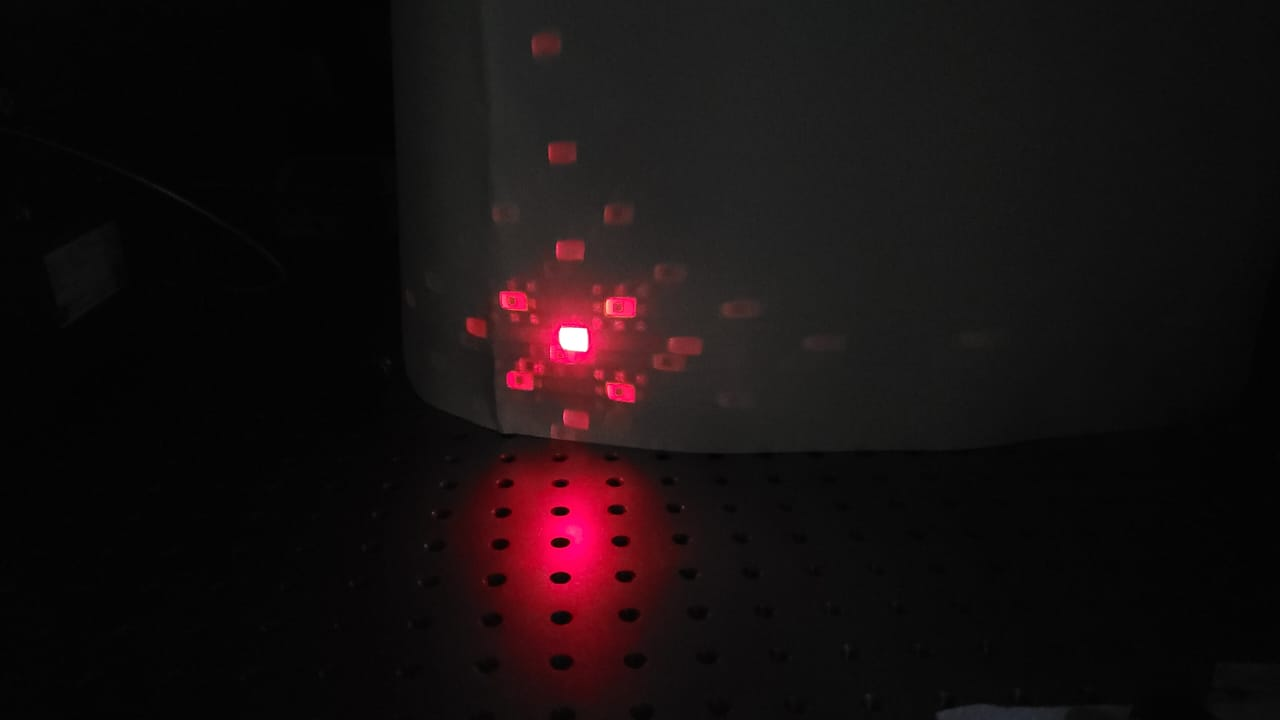
\includegraphics[width=0.9\textwidth]{img/diff.jpeg}
\caption{Diffraction Order after beam get modulated from the SLM}
\end{figure}

\vspace{1 cm}

\begin{figure}[H]
\label{img: result}
\centering
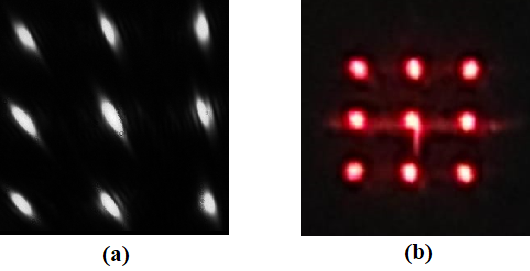
\includegraphics[width=0.9\textwidth]{img/result_img.png}
\caption{(a) Optical Tweezers imaged through CMOS Camera, (b) Optical Tweezers imaged on the screen}
\end{figure}

\vspace{0.5 cm}
We have also analysed the intensity distribution of the tweezers shown in Figure 8(a). The imaged intensity follows the gaussian pattern in both horizontal and vertical directions of traps, as depicted in figure 9. The shape is not circular, and the intensity of each trap is slightly different, maybe because we are using the circular aperture to block the diffraction orders. Imaging the focal plane of the lens without the iris gave us circular-shaped tweezers. So using a rectangular aperture for filtering instead of a circular might be beneficial.

\begin{figure}[H]
\label{img:intensity analysis}
\centering
\includegraphics[width=\textwidth]{img/20220831_4_Profile.png}
\caption{Analysis of intensity pattern of each rows and columns for the Optical Tweezers arrays of Figure 8(a)}
\end{figure}
%--------------------------------------------------------------------------------
\vspace{1.1 cm}

\subsection{Defect free array formation}
\label{subsec: defect free array}
Since the atom is not trapped yet, we have tried to simulate the trapped atom configuration by randomly generated the optical tweezers pattern. Figure 10(a) shows the randomly generated trapped configuration $(I = \{x_i, y_i\})$ with a load probability of 50 percent for each site and 10(b) shows the plot for the final configuration of atom $(T = \{a_i, b_i\})$. After implementing the Hungarian algorithm on the bipartite graph $G(I, T, E)$, we obtain the matching shown in figure 11. Experimental demonstration of optical tweezers movement is shown in figure 12 and 13.

\begin{figure}[H]
\label{fig:tweezers_plot}
\centering
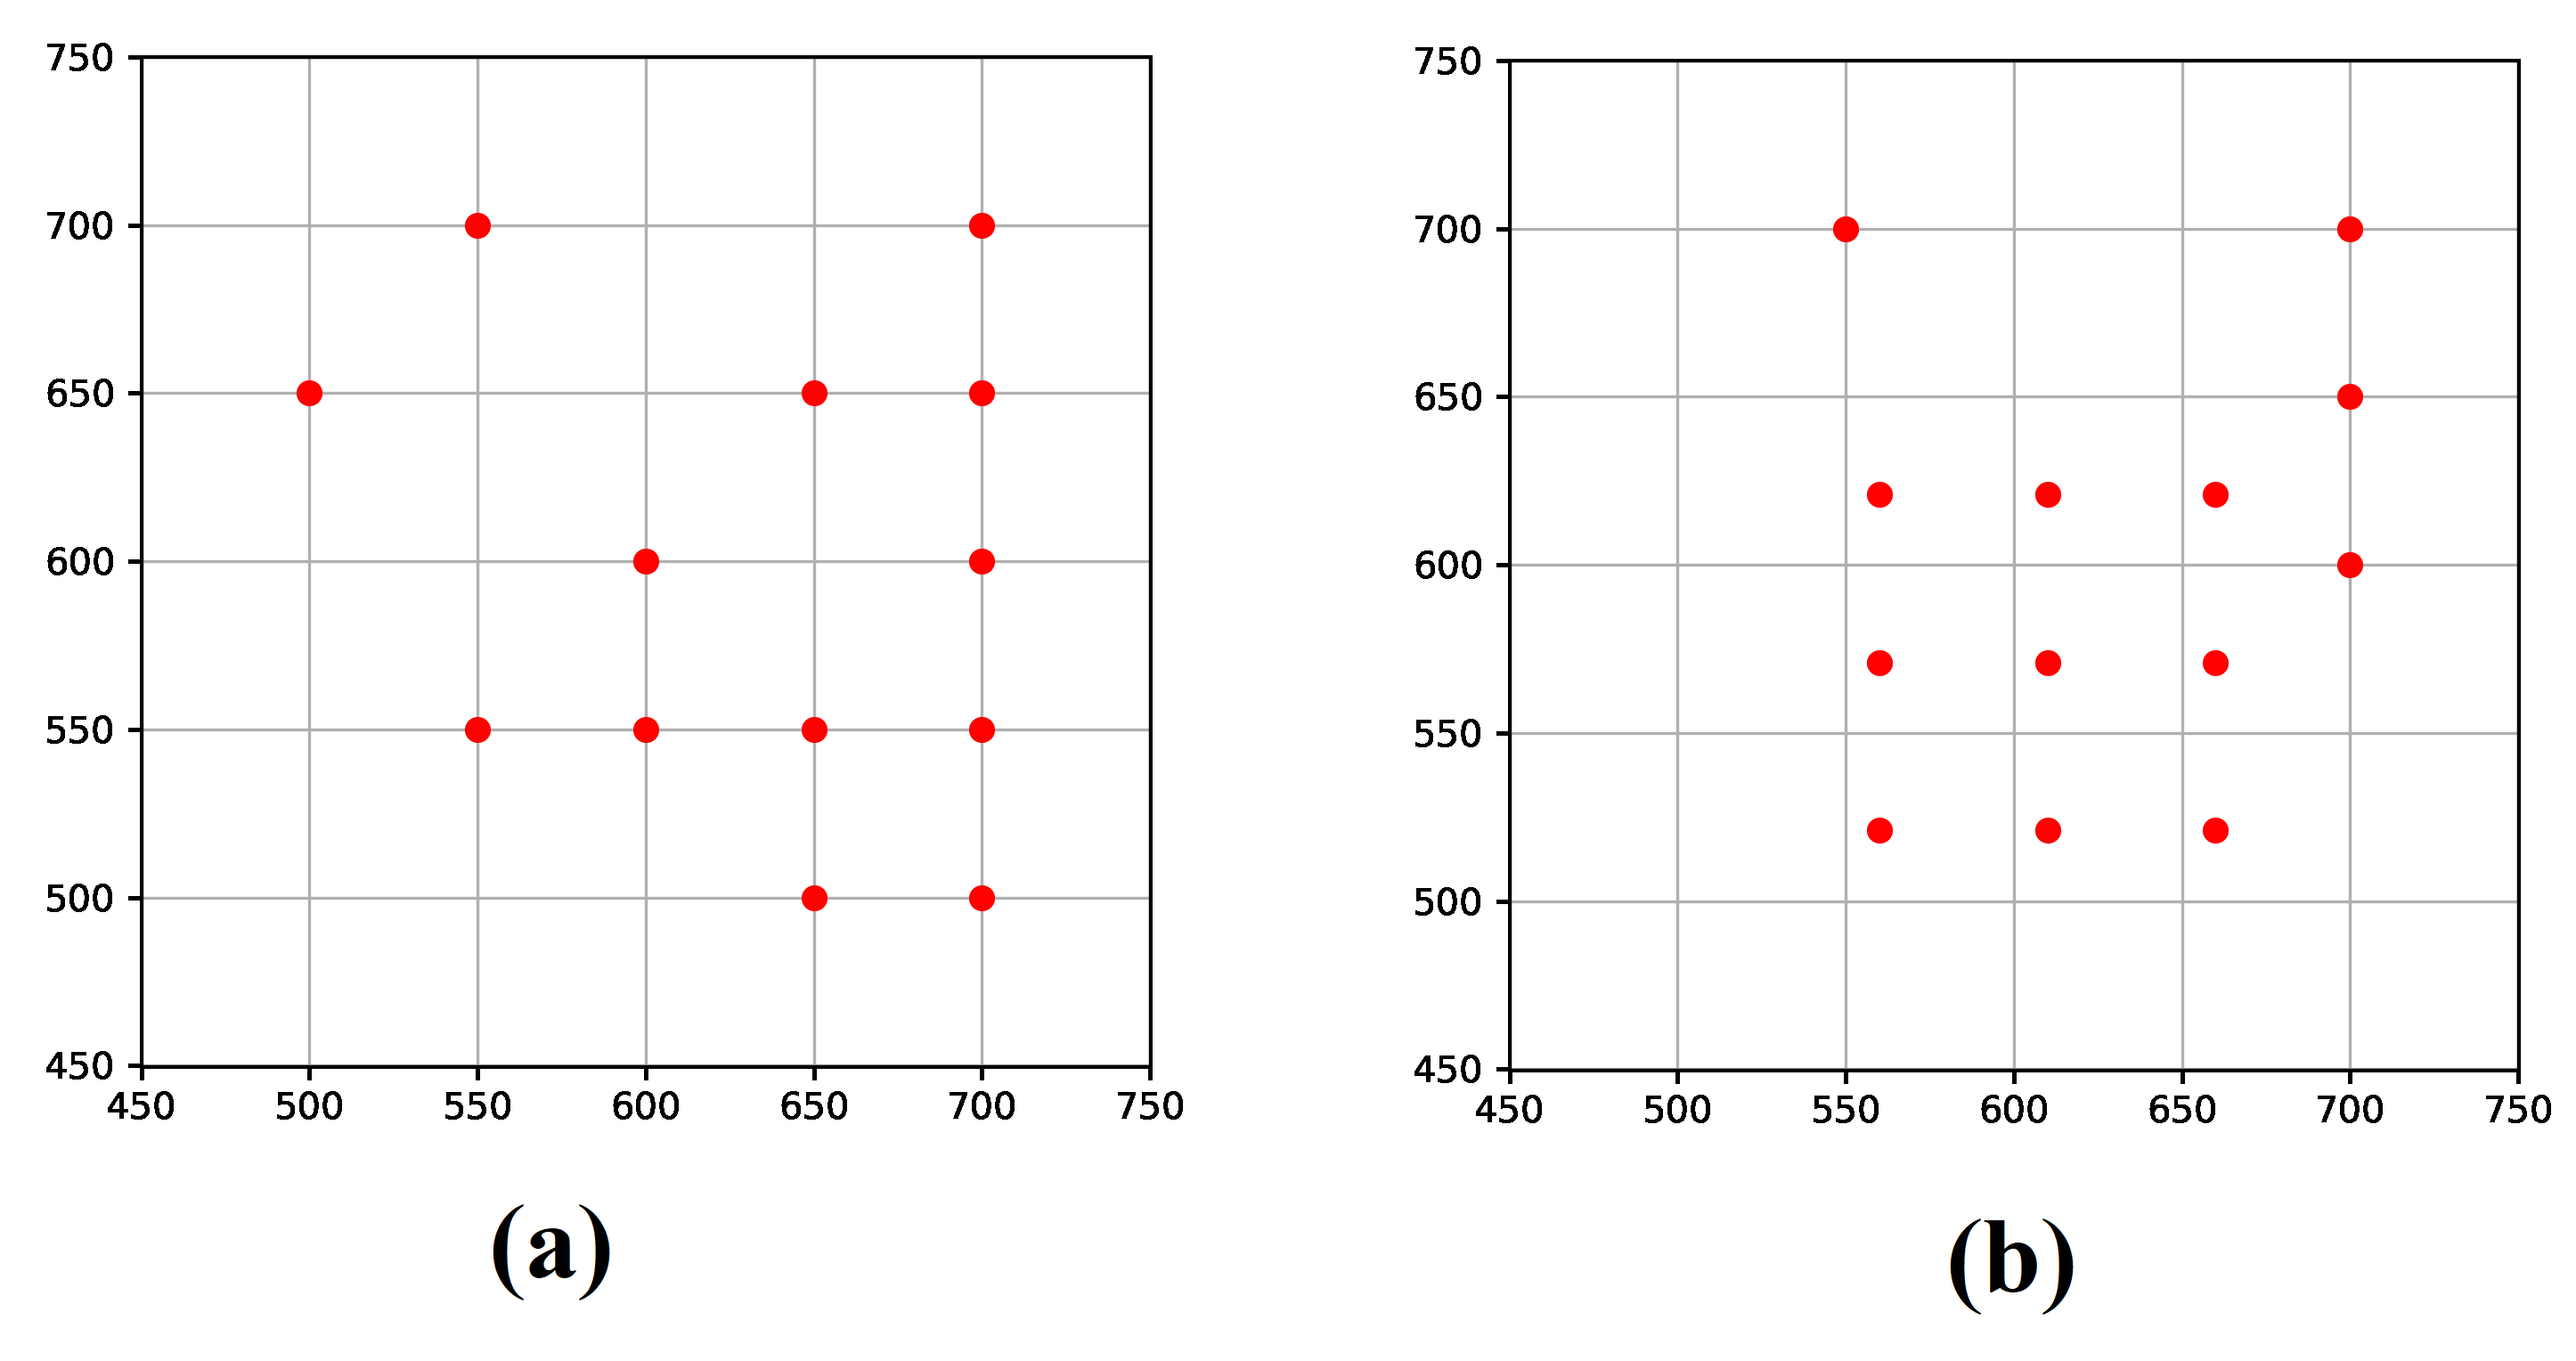
\includegraphics[width=\textwidth]{img/tweezers_plot.png}
\caption{(a) Initial configuration of trapped array, (b) Final configuration of trapped array}
\end{figure}

\begin{figure}[H]
\label{fig:combined_move}
\centering
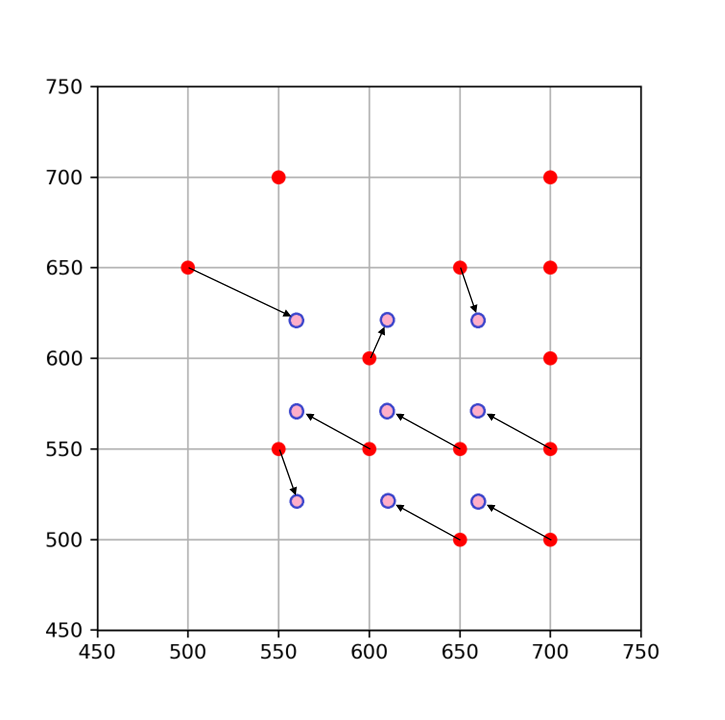
\includegraphics[width=0.65\textwidth]{img/combined_move.png}
\caption{Illustrations of the moves from an initial $5 \times 5$ array to a final $3 \times 3$ array. Simulation can be seen \href{https://drive.google.com/file/d/1JTKyHGn4GLYZHJFvZTr1iKvnrk_kMZGr/view?usp=share_link}{here}.}
\end{figure}

\vspace{0.5cm}
\begin{figure}[H]
\label{trap_slm}
\centering
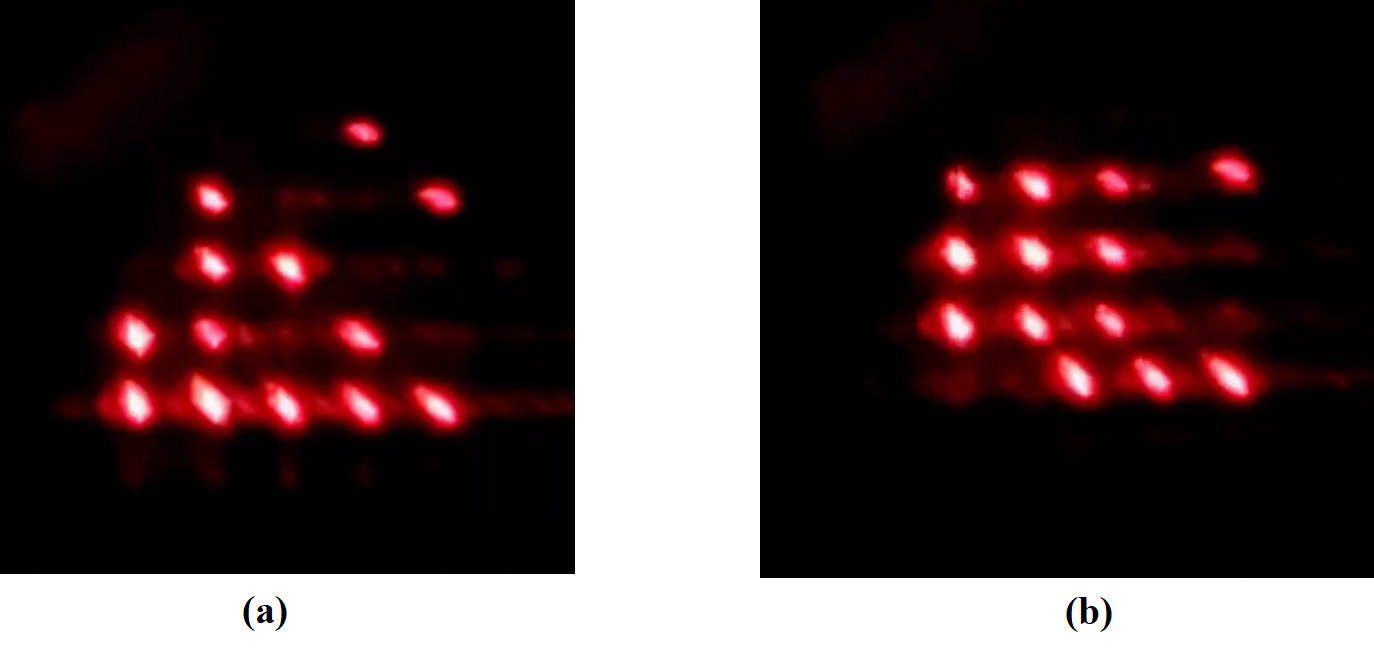
\includegraphics[width=0.9\textwidth]{img/tweezers.png}
\caption{(a) Initial configuration of trapped atom and (b) Final configuration of atom in array projected on screen}
\end{figure}

\vspace{0.8cm}
\begin{figure}[H]
\label{frames}
\centering
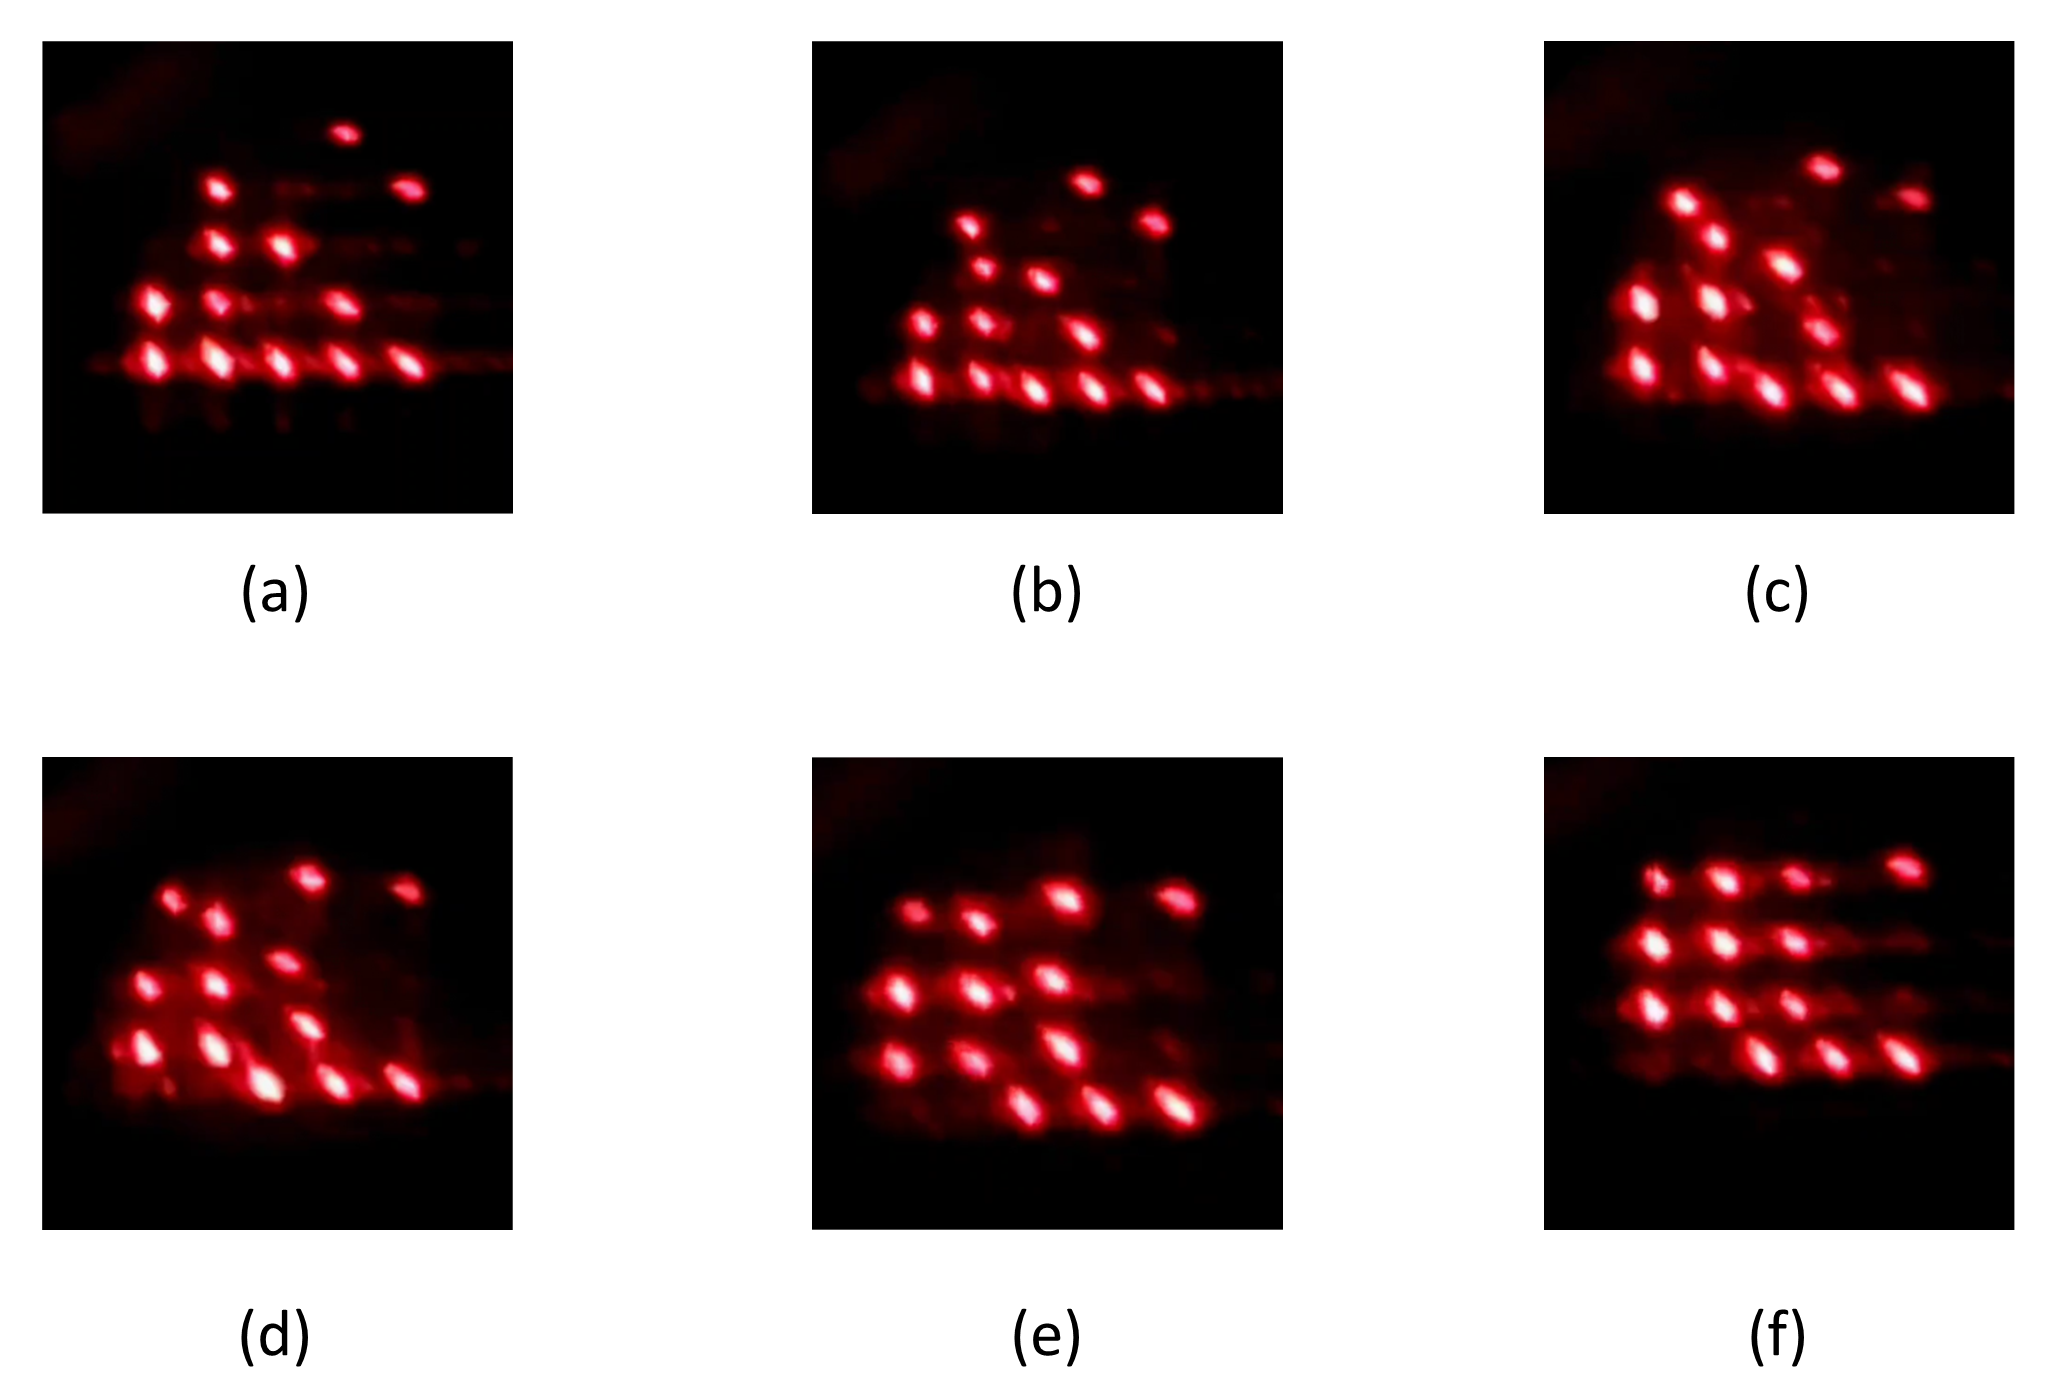
\includegraphics[width=\textwidth]{img/frame.png}
\caption{Snapshots of the frames during the movement. (a) initial frame, (b), (c), (d) and (e) are frames in between the movement and (f) is the final frame. Entire movement of optical tweezers can be seen \href{https://drive.google.com/file/d/10Ov5Z4IybwpwF9MXvInDwmm_61tb9SZ2/view?usp=sharing}{here}.}
\end{figure}

% The trapped atom configuration is generated randomly as per now.